\documentclass[11pt,article,oneside]{article}

\usepackage[final,nonatbib]{neurips_2024}

% Colors
\usepackage[dvipsnames]{xcolor}

% ===============
% Hyperlink setup
% ===============
\usepackage{xurl}
\usepackage[
    colorlinks,
    breaklinks=true,
    urlcolor=NavyBlue,
    citecolor=NavyBlue,
    linkcolor=NavyBlue,
    linktocpage,
]{hyperref}
\def\sectionautorefname{\S}
\def\subsectionautorefname{\S}

% Nicer monospace font
\usepackage{inconsolata}

% Using Palatino for text and math
\usepackage{newpxtext}
\usepackage{newpxmath}

% Improved typography
\usepackage{microtype}

\usepackage{graphicx}
\usepackage{algorithm}
\usepackage{algpseudocode}
\usepackage{array}
\usepackage{caption}
\usepackage{geometry}
\usepackage{amsmath}
\usepackage{hyperref}
\usepackage{inconsolata}
\usepackage{newpxtext}
\usepackage{newpxmath}
\usepackage{microtype}
\usepackage{booktabs}

% Bibliography setup
\usepackage[
    natbib,
    style=numeric-comp,
    sorting=none,
    doi=false,
    isbn=false,
    url=true,
    eprint=false,
    maxbibnames=10,
    hyperref
]{biblatex}
\addbibresource{bibliography.bib}
\renewcommand\bibfont{\small}
\newbibmacro{string+doiurlisbn}[1]{%
  \iffieldundef{doi}{%
    \iffieldundef{url}{%
      \iffieldundef{isbn}{%
        \iffieldundef{issn}{%
          #1%
        }{%
          \href{http://books.google.com/books?vid=ISSN\thefield{issn}}{#1}%
        }%
      }{%
        \href{http://books.google.com/books?vid=ISBN\thefield{isbn}}{#1}%
      }%
    }{%
      \href{\thefield{url}}{#1}%
    }%
  }{%
    \href{http://dx.doi.org/\thefield{doi}}{#1}%
  }%
}

\DeclareFieldFormat[article,book,incollection,inproceedings,data]{title}%
    {\usebibmacro{string+doiurlisbn}{#1}}

\DeclareFieldFormat*{url}{}
\DeclareFieldFormat[online]{url}{\mkbibacro{URL}\addcolon\space\url{#1}}

\DeclareFieldFormat[misc]{title}{\usebibmacro{string+doiurlisbn}{\mkbibemph{#1}}}


\title{Detecting Financial Fraud: Leveraging Machine Learning for
Enhanced Security and Loss Prevention}
\author{
    Usama Ahmed\\
    School of Information \\
    University of Arizona\\
    \texttt{usamaahmed@arizona.edu}
}
\begin{document}
\maketitle

\section{Introduction}

Fraudulent activities are illegal practices in which an individual or system deceives another for personal gain \cite{fraud1}. 
Among these, financial frauds such as credit card frauds involve deceiving an individual to obtain their personal information, 
including security pins. To reduce financial losses and enhance user security in financial systems, the aim was to develop a robust 
model that can detect fraudulent activities and distinguish them from genuine transactions. The dataset \cite{dataset} used in this 
project is sourced from Kaggle and was uploaded by Gabriel Pedra. It contains transactions made by European cardholders in September
2023.

At present, the detection of fraudulent activity is primarily dependent on rule-based systems - predetermined if-else statements
that assess input data and initiate responses \cite{7735}. Yet, these systems encounter significant obstacles when it comes
to detecting irregularities in transaction patterns. Essentially, any behavior that falls outside their if-else statements 
will not be recognized as an anomaly \cite{7735}.  

To address these challenges, this project introduced a cutting-edge solution that harnesses the power of machine learning 
algorithms, specifically those that detect anomalies \cite{c2}. Python libraries such as scikit-learn, numpy, pandas, and matplotlib 
to effectively manage the data, visualize it, and create classification models were used. Support Vector Machines (SVM) was  
the main machine learning model utilized due to its ability to handle imbalanced datasets. The effectiveness of this model was
evaluated using a range of key metrics including precision, recall, and F1-score \cite{c2}.

The model achieved high precision (1.00) for real transactions (class 0) but a slightly lower precision (0.79) for 
fraudulent transactions, indicating accurate classification with a trade-off in detecting fraud.

The impact of this project goes beyond technological advancement. It stands to benefit a diverse group of stakeholders, 
including financial institutions, businesses, and consumers. By reducing financial losses and improving operational efficiency, 
companies are empowered to operate at their best \cite{7735}. This model also enhances user security and has the potential to 
revolutionize labor dynamics. Currently, many companies hire resources to detect financial fraud. Building a model 
like this frees up valuable resources, allowing them to focus on more high-value tasks \cite{7735}.



\section{Methods}

The dataset contains credit card transactions made by European cardholders in September 2013. 
It consists of numerical input variables resulting from a PCA transformation. The dataset \cite{dataset} 
includes features such as Time, V1-V28 (principal components), Amount, and Class (0 for non-fraudulent, 1 for fraudulent). 
The dataset contains 284807 rows and 31 columns, with the rows representing the number of transactions that occured in two days.
Out of the 284807 transactions, only 497 were frauds, therefore the dataset is highly imbalanced
An example training data point from the dataset is shown below:

\begin{verbatim}
    Time: 0
    V1: -1.359807
    V2: -0.072781
    ...
    Amount: 149.62
    Class: 0 (non-fraudulent)
    \end{verbatim}

\subsection{Support Vector Machine (SVM)}
 Support Vector Machines (SVM) were used to classifiy fraudulent transactions. SVMs represent a supervised learning algorithm 
 category applicable to classification or regression tasks. Their core concept involves identifying a hyperplane that effectively distinguishes between various classes within 
 the training dataset. The objective is to locate the hyperplane with the greatest margin, defined as the distance 
 between the hyperplane and the nearest data points of each class. This determined hyperplane facilitates the classification
 of new data by assessing its position relative to the hyperplane. SVMs prove advantageous in scenarios with numerous 
 features in the data or when a distinct separation margin exists between classes \cite{SVMdef}.  


  
  Here is the pseudocode of the algorithm:

\begin{algorithm}
    \caption{TrainSVM}
    \begin{algorithmic}[1]
        \Procedure{TrainSVM}{$x_{\text{train}}, y_{\text{train}}, C_{\text{values}}, \text{kernel\_types}, num_{\text{folds}}$}
            \State Initialize an empty list to store the performance metrics of each model
            \For{\textbf{each} $C$ \textbf{in} $C_{\text{values}}$}
                \For{\textbf{each} $\text{kernel\_type}$ \textbf{in} $\text{kernel\_types}$}
                    \State Initialize an SVM model grid search with hyperparameters $C = 1, 10, 100$ and $\text{kernel\_type} = \text{linear , rbf}$
                    \State Initialize an empty list to store performance metrics for each fold
                    \For{$\text{fold} = 1$ \textbf{to} $num_{\text{folds}}$}
                        \State Split the training data into training and validation sets using k-fold CV
                        \State Train the SVM model on the training set $(x_{\text{train}}, y_{\text{train}})$
                        \State Evaluate the model on the validation set and calculate performance metrics
                        \State Add the performance metrics to the list of fold metrics
                    \EndFor
                    \State Calculate the average performance metrics of the current model over all folds
                    \State Add the average performance metrics to the list of model metrics
                \EndFor
            \EndFor
            \State Identify the model with the best average performance metrics
            \State Train the SVM model with the best hyperparameters on the entire training data
            \State \textbf{return} the trained SVM model with the best hyperparameters
        \EndProcedure
    \end{algorithmic}
    \end{algorithm}
        

\subsection{Evaluation Procedure}
The performance of the model was evaluated using metrics such as precision, recall, and F1-score. 

Precision measures the accuracy of positive predictions made by the classifier (SVM). 

\[
\text{Precision} = \frac{\text{True Positives}}{\text{True Positives} + \text{False Positives}}
\]

Recall (or Sensitivity) measures the ability of the classifier to measure all positive instances 

\[
\text{Recall} = \frac{\text{True Positives}}{\text{True Positives} + \text{False Negatives}}
\]

F1-score is the harmonic mean of precision and recall. It provides a balance between precision and recall

\[
\text{F1 Score} = 2 \times \frac{\text{Precision} \times \text{Recall}}{\text{Precision} + \text{Recall}}
\]


Furthermore, cross-validation was used to ensure robustness of the results.
    
\subsection{Hyperparameter Tuning}
Grid search was employed to tune the hyperparameters of the SVM model, such as the regularization parameter (C), 
kernel (linear, rbf), and gamma (scale, auto)
    


\section{Results}

\begin{figure}[!htb]
    \centering
    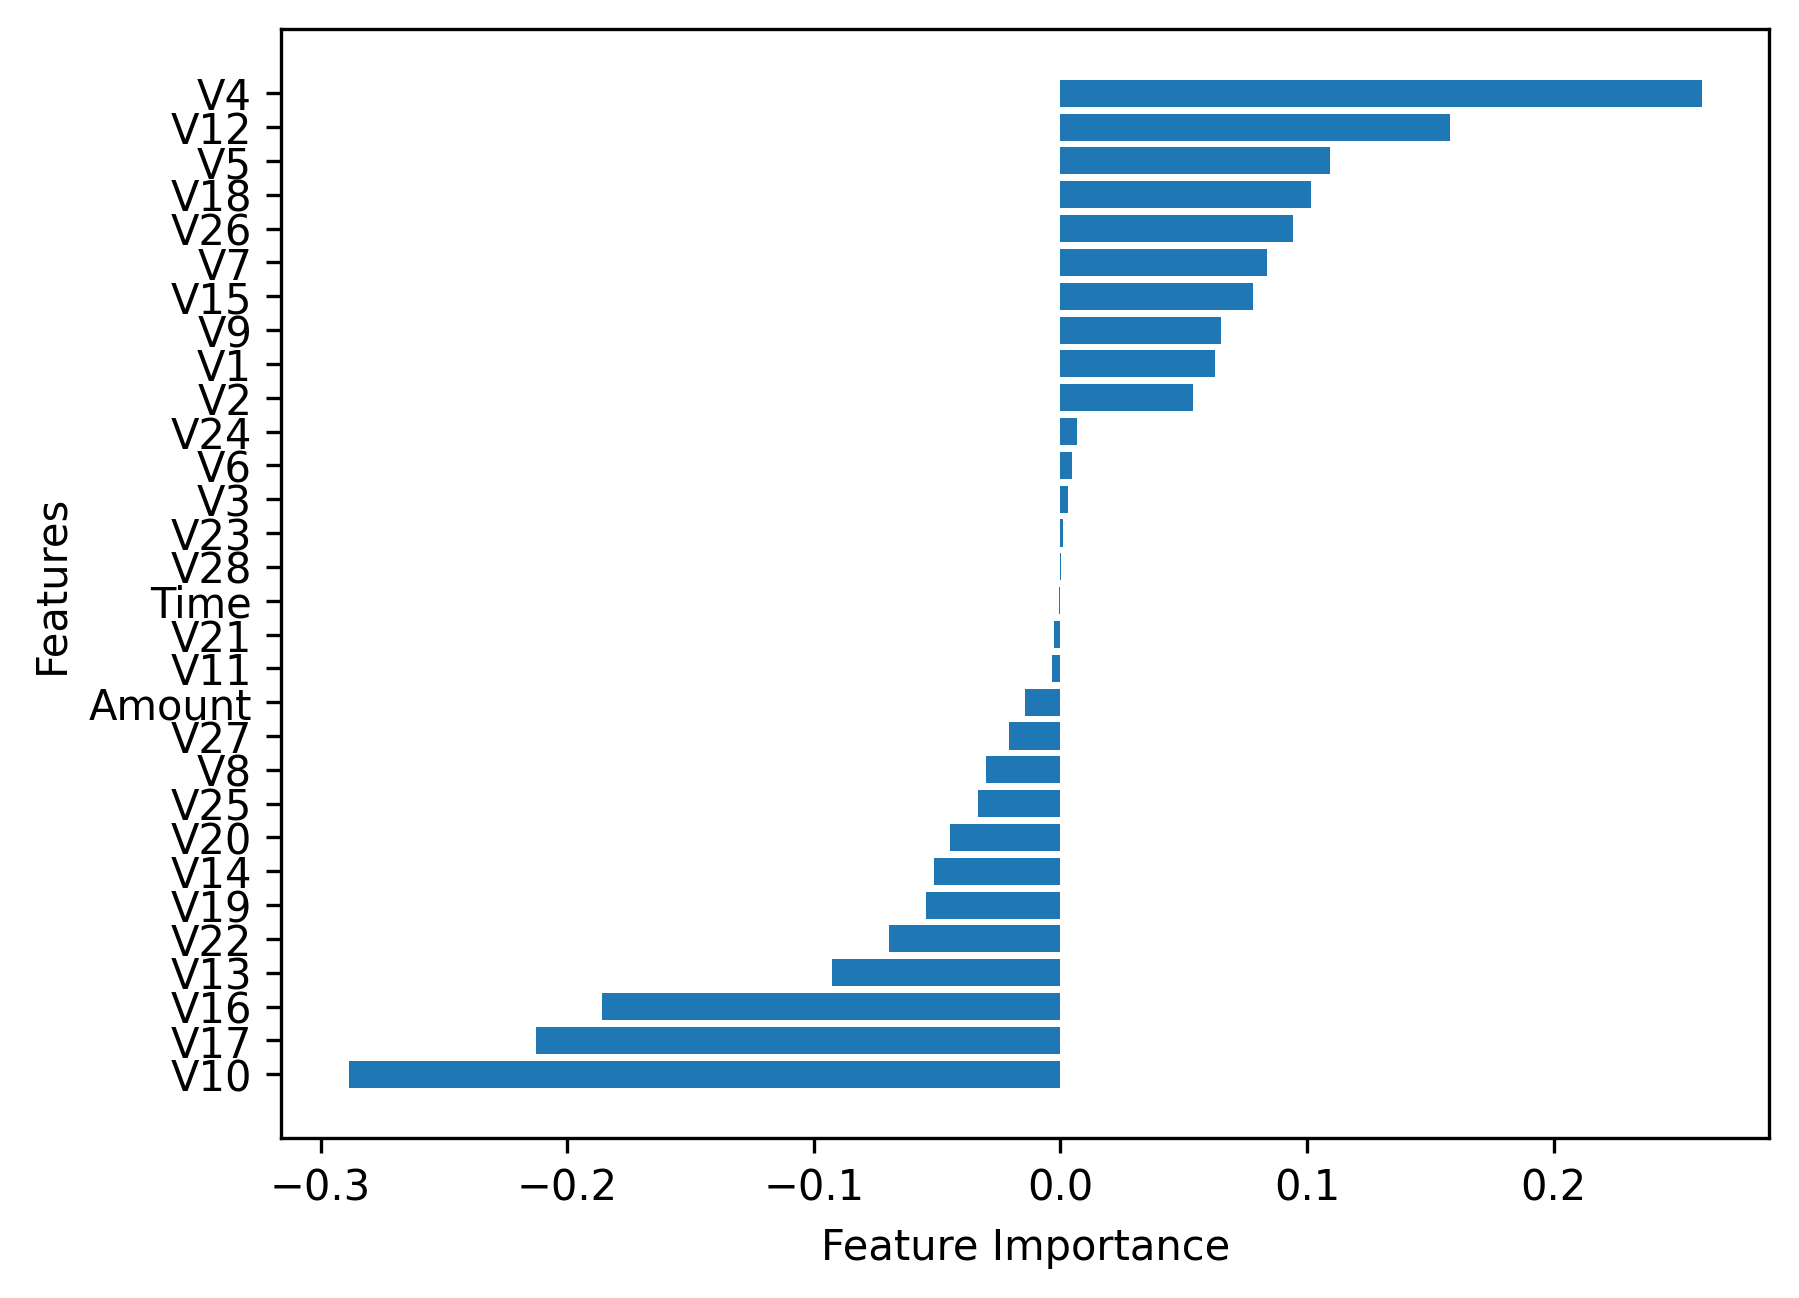
\includegraphics[width=0.7\linewidth]{feature_importance.png}
    \caption{Features V4, V12, and V5 strongly predict fraudulent transactions (Class 1), with higher values indicating genuine
     transactions. Conversely, V17, V16, and V10 are significant for real transactions, with lower values signaling fraud. 
     'Amount' and 'Time' have minor importance, implying they don't significantly aid class differentiation in the model.}
    \label{Fig 1: Feature Importance}
\end{figure}

    
    \begin{table}[H]
        \centering
        \caption{Classification Report}
        \label{tab:best_model_classification_report}
        \begin{tabular}{@{}lcccc@{}}
        \toprule
        Class & Precision & Recall & F1-Score & Support \\ \midrule
        Real     & 1.00      & 1.00   & 1.00     & 56864   \\
        Fraudulent     & 0.79      & 0.79   & 0.79     & 98      \\ \midrule
        Accuracy & \multicolumn{3}{c}{\hspace{3cm} 1.00} & \\ \midrule
        \end{tabular}
    \end{table}
    
    
    The model's performance metrics reveal a precision of 1.00 for class 0 (real transactions) and 0.79 for class 1 
    (fraudulent transactions), indicating accurate positive predictions but a slight trade-off in identifying fraudulent transactions.
    The recall scores of 1.00 for class 0 and 0.79 for class 1 showcase the model's ability to correctly identify genuine transactions
    but with a similar trade-off in identifying fraudulent ones. The F1-scores, a balance of precision and recall, stand at 1.00 for 
    class 0 and 0.79 for class 1, demonstrating strong performance overall with a consideration of trade-offs. With 56,864 
    instances of class 0 and 98 instances of class 1, the model's accuracy reaches 1.00.
    
    \begin{table}[H]
    \centering
    \caption{Confusion Matrix}
    \begin{tabular}{|c|c|c|}
    \hline
    True\textbackslash Predicted & 0 & 1 \\
    \hline
    0 & 56843 & 21 \\
    1 & 21 & 77 \\
    \hline
    \end{tabular}
    \end{table}
    
    The confusion matrix offers a granular view of a model's predictions, distinguishing between True Negatives (0,0), 
    False Positives (0,1), False Negatives (1,0), and True Positives (1,1). In this case, there were 56,843 True Negatives, 
    indicating instances correctly identified as genuine transactions. The model also had 21 False Positives, where transactions 
    were inaccurately labeled as fraudulent when they were not. Conversely, there were 21 False Negatives, representing genuine 
    transactions misclassified as fraudulent. Finally, the model accurately identified 77 instances as True Positives, correctly 
    flagging them as fraudulent transactions. 
    

\section{Discussion}

\begin{figure}[!htb]
    \centering
    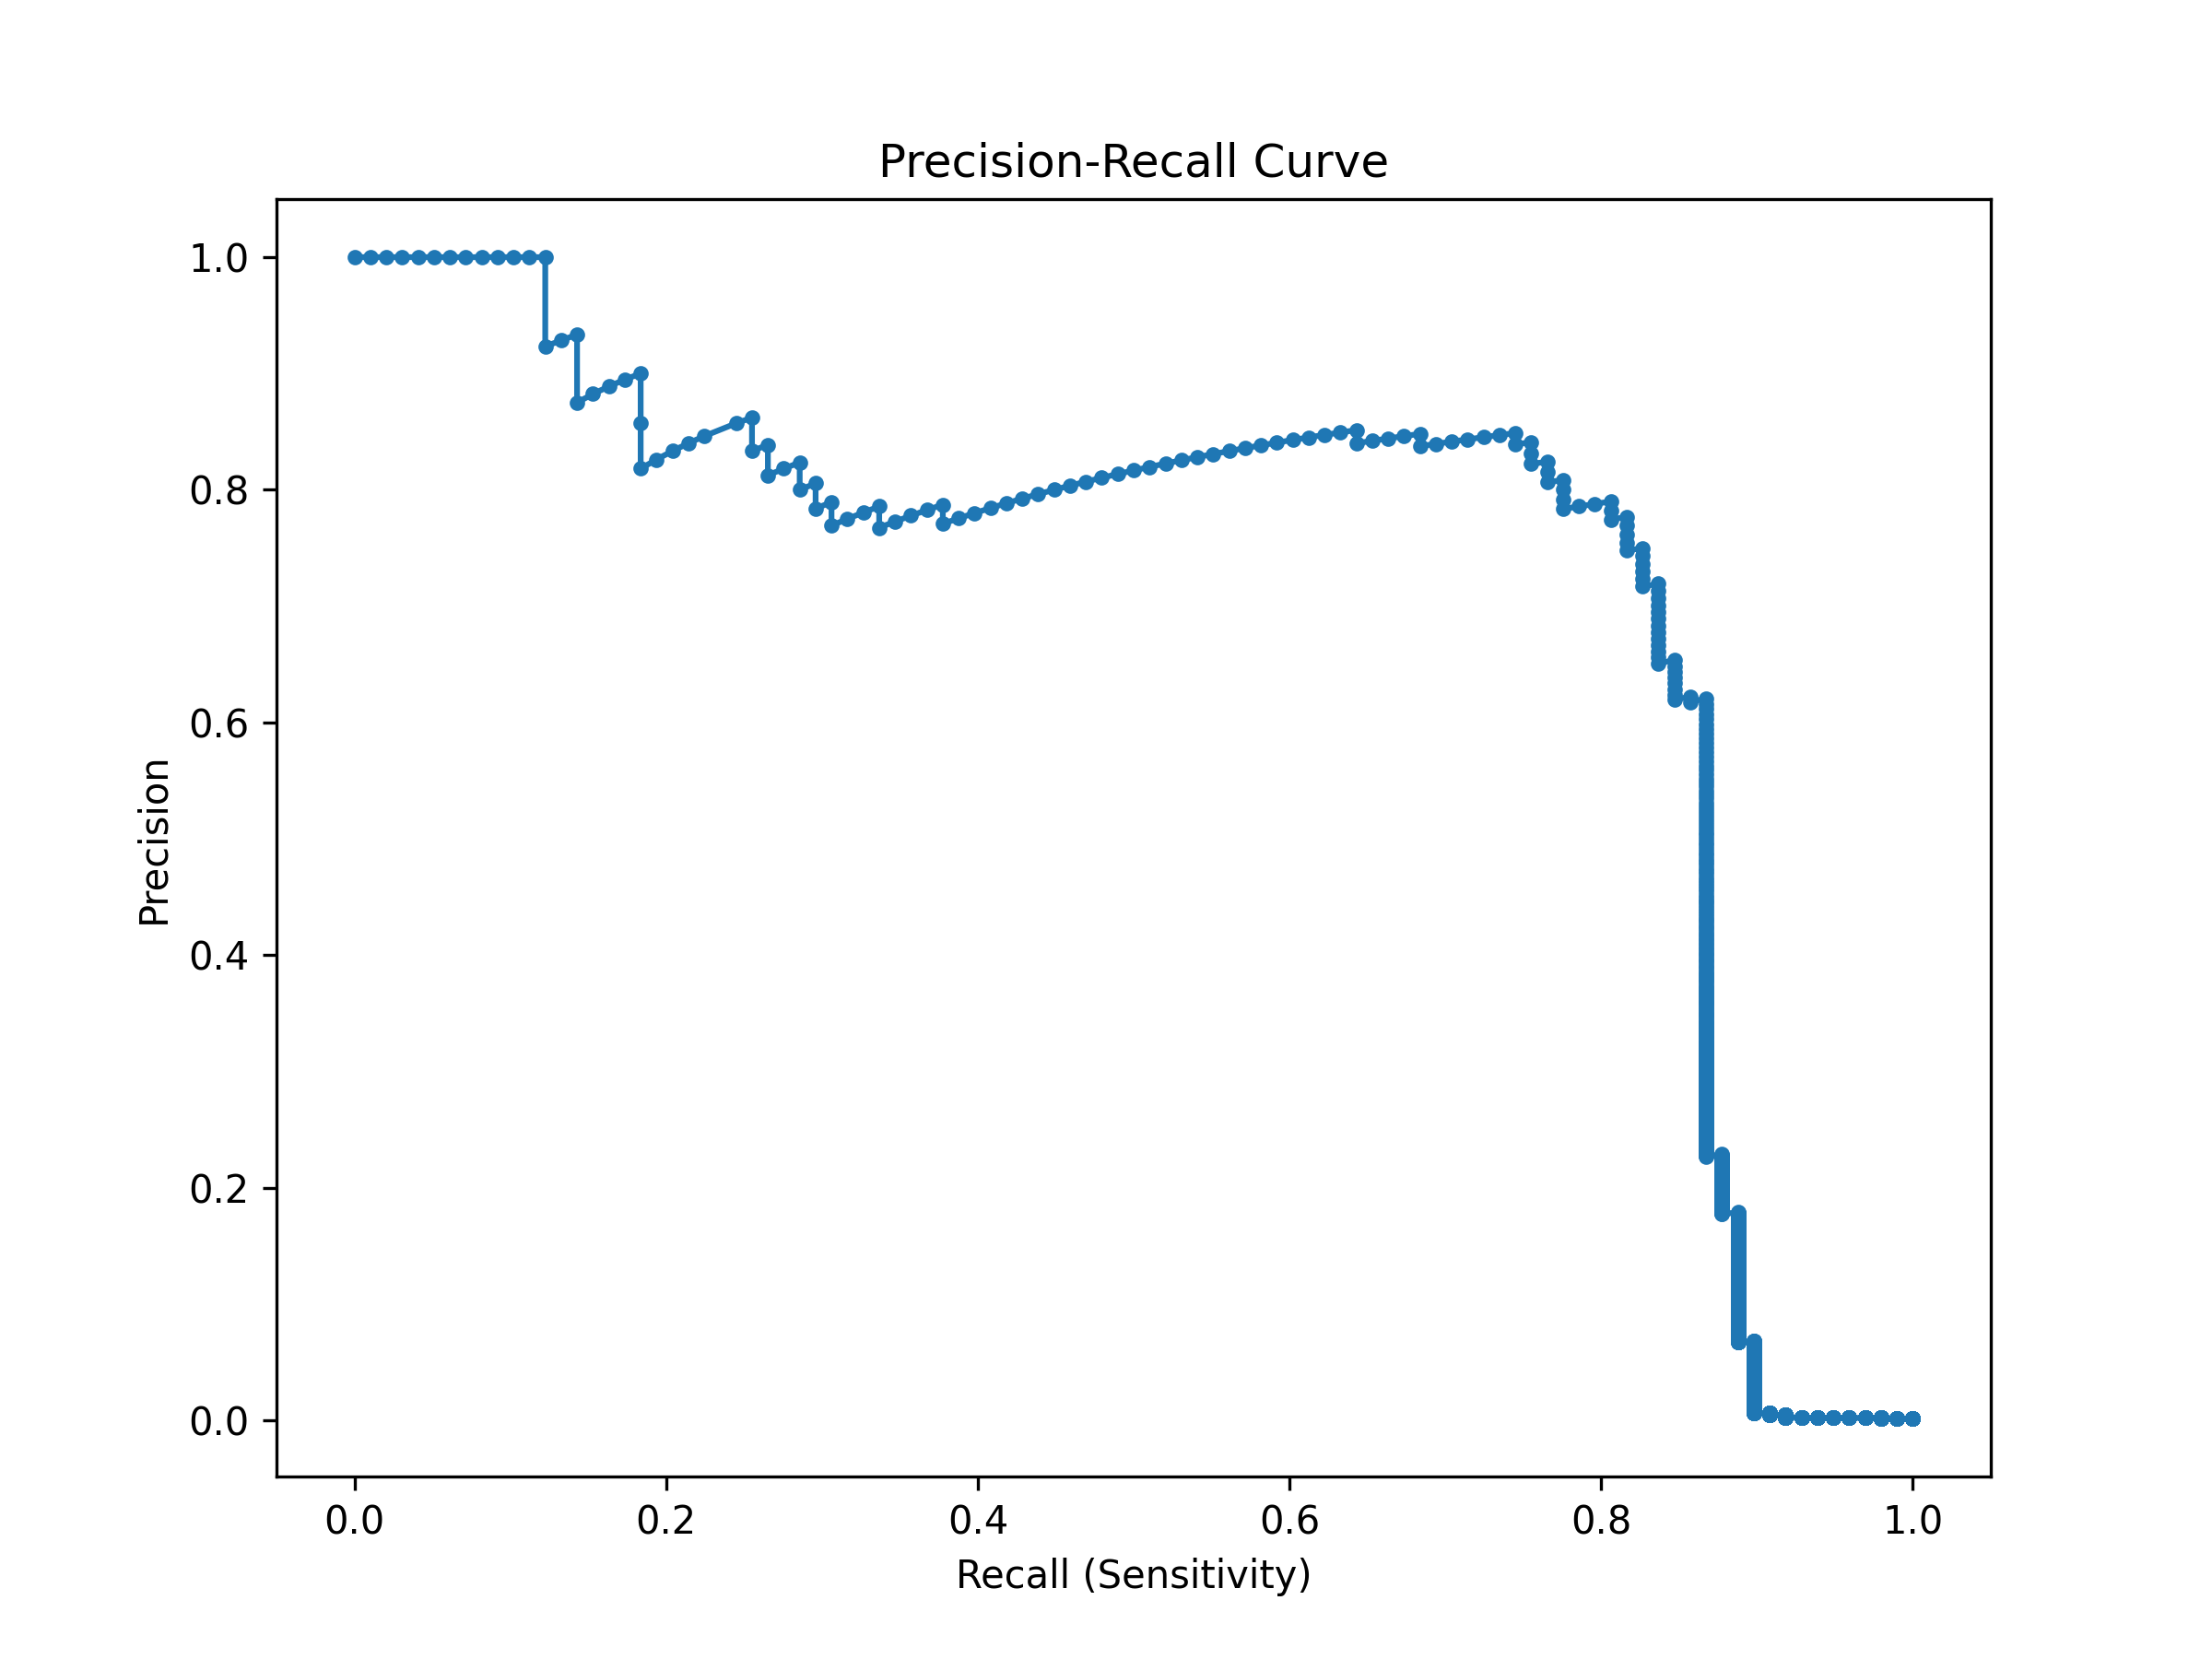
\includegraphics[width=0.7\linewidth]{precision_recall_curve.png}
    \caption{The precision-recall curve shows how the model's precision and recall change with different 
    classification thresholds. Initially, high precision suggests accurate predictions but possibly misses some 
    positives. As recall increases, precision decreases due to more false positives. The curve's steps indicate 
    critical thresholds where small gains in recall lead to significant drops in precision, emphasizing the need for
    a balanced approach in fraud detection models.}
    \label{Fig 2:Precision Recall Curve}
\end{figure}


The precision-recall curve shows how the model's precision and recall change with different classification thresholds. 
Initially, high precision suggests accurate predictions but possibly misses some positives. As recall increases, 
precision decreases due to more false positives. The curve's steps indicate critical thresholds where small gains in recall 
lead to significant drops in precision, emphasizing the need for a balanced approach in fraud detection models.
    
    
The results from the classification report and confusion matrix demonstrate the effectiveness of the model in fraud detection. 
The high precision of 1.00 for genuine transactions indicates that the model rarely misclassifies legitimate transactions as 
fraudulent. However, for fraudulent transactions, the precision of 0.79 suggests that approximately 79 of transactions 
flagged as fraudulent are indeed fraudulent. This trade-off between precision and recall in class 1 reflects the challenge 
of handling class imbalance. Moreover, since real transactions (Class 0) significantly outnumber the fraudulent class (Class 1),
the SVM classifier achieves high accuracy (1.00) by simply predicting the majority class most of the time. 
    
For class imbalance, various sampling techniques like SMOTE and class weights were used, but these approaches 
could not completely fix the problem. While these techniques offered a high recall score, they often led to a lower 
precision score. This discrepancy occurred because the synthetic samples generated by SMOTE and the adjusted class weights 
focused more on capturing minority class instances, thus increasing recall but sometimes at the expense of precision \cite{rnd1}.  

\printbibliography

\end{document}
